%----------------------------------------------------------------------------------------
%	CHAPTER 5
%----------------------------------------------------------------------------------------
\chapterimage{ChapterImages/chapter5.png} % Chapter heading image

\chapter{Shell Programming I}
\label{ch:shell1}

Shell scripting is a fundamental skill for system administrators and advanced Linux users. It lets you automate repetitive tasks, manage system operations, and build powerful tools simply by combining the commands you already know from Chapter~\ref{ch:textfiles} and Chapter~\ref{ch:users-groups}.

\section{What is a Shell?}
The shell is a command-line interface (CLI) that acts as an intermediary between the user and the operating system kernel. It provides several key capabilities:
\begin{itemize}
    \item Interactive command execution for file navigation and process management.
    \item Scripting capabilities that allow automation of complex tasks.
    \item Command piping and redirection for combining multiple operations.
\end{itemize}
The shell is the outermost layer surrounding the operating system: it interprets the commands and scripts you type and translates them into requests the kernel can act on. Figure~\ref{fig:shell-stack} shows where it sits relative to the kernel and the hardware.

\begin{figure}[h]
    \centering
    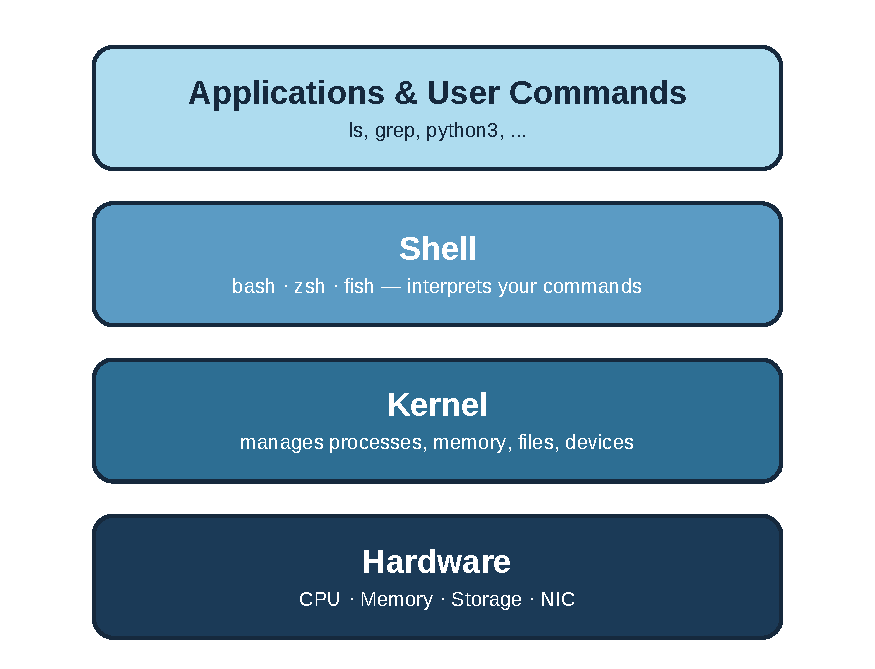
\includegraphics[width=0.6\textwidth]{Images/Chapter5/shell-system-stack.pdf}
    \caption{The shell's place in the system: it sits between the applications you run and the kernel that manages the hardware.}
    \label{fig:shell-stack}
\end{figure}

\section{Types of Shells}
Linux systems support multiple shell implementations, each with unique features:
\begin{itemize}
    \item \texttt{bash} --- Bourne Again Shell, the default on most modern Linux systems.
    \item \texttt{sh} --- the original Bourne shell, predecessor to \texttt{bash}.
    \item \texttt{zsh}, \texttt{fish}, \texttt{csh} --- alternative shells offering additional features and customizations.
\end{itemize}
All available shell interpreters are listed in the \texttt{/etc/shells} file.

\section{Shell Interpreter Working Modes}
Shell interpreters operate in two distinct modes:
\begin{itemize}
    \item \textbf{Interactive mode} --- the interpreter interacts directly with the user, accepting commands and displaying results in real time.
    \item \textbf{Non-interactive mode} --- the interpreter executes commands from a script file without user interaction.
\end{itemize}

\textbf{How to Run a Shell Script:}
\begin{enumerate}
    \item Open a text editor and write your shell commands. Save the file with a \texttt{.sh} extension (for example, \texttt{myscript.sh}).
    \item Run the script, using either method:
\begin{lstlisting}[language=Terminal]
$ bash myscript.sh
\end{lstlisting}
    or make it executable and run it directly:
\begin{lstlisting}[language=Terminal]
$ chmod +x myscript.sh
$ ./myscript.sh
\end{lstlisting}
\end{enumerate}

\section{Shell Scripts}
A shell script is a text file containing a series of shell commands executed sequentially by the shell interpreter.

\textbf{Basic Script Structure:}
\begin{lstlisting}[language=Terminal]
#!/bin/bash
# My first script
echo "Hello, $USER"
echo "Today is $(date)"
\end{lstlisting}

The first line \texttt{\#!/bin/bash} (called a \emph{shebang}) tells the OS to use \texttt{bash} as the interpreter. Lines beginning with \texttt{\#} are comments. The script uses the variable \texttt{\$USER} and command substitution \texttt{\$(date)} to display dynamic information. Figure~\ref{fig:script-anatomy} breaks this example down line by line.

\begin{figure}[h]
    \centering
    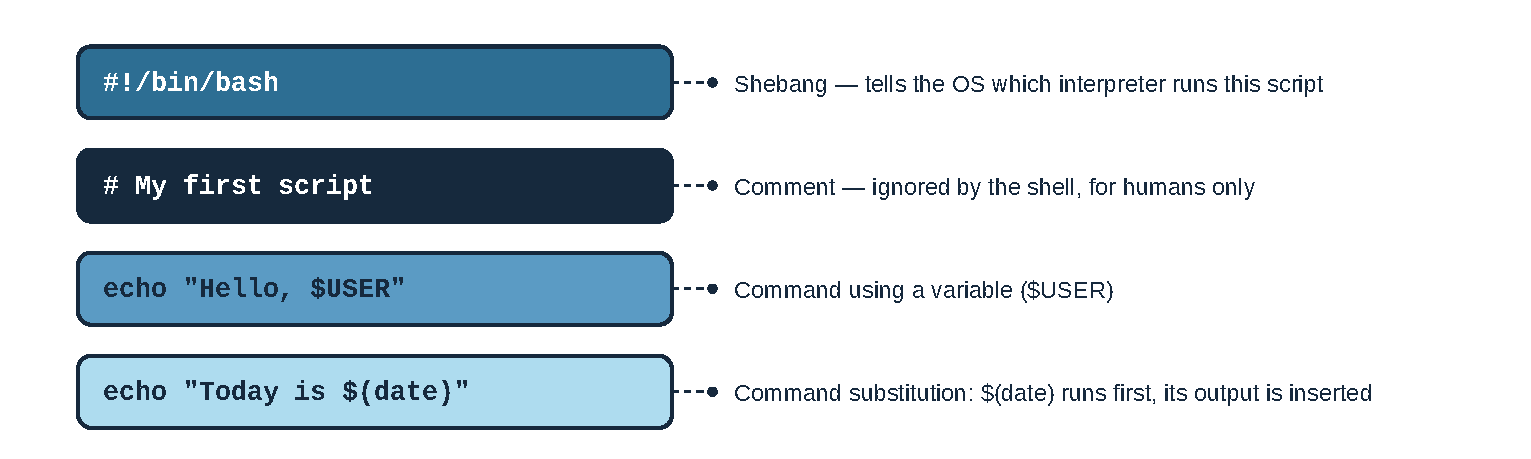
\includegraphics[width=\textwidth]{Images/Chapter5/script-anatomy.pdf}
    \caption{Anatomy of a simple shell script.}
    \label{fig:script-anatomy}
\end{figure}

\section{Variables}
Variables store data values that can be referenced and manipulated throughout a script.

\textbf{Basic Assignment:}
\begin{lstlisting}[language=Terminal]
#!/bin/bash
variable_name=value
\end{lstlisting}
\textbf{Important:} No spaces are allowed around the equals sign; spaces act as delimiters in the shell.

\textbf{Accessing Variables:}\\
Use the \texttt{\$} prefix to retrieve a variable's value:
\begin{lstlisting}[language=Terminal]
#!/bin/bash
x=4
echo $x          # Outputs: 4
echo $undefined  # Outputs: empty string
\end{lstlisting}
Undefined variables produce empty strings rather than errors.

\textbf{Performing Arithmetic:}\\
By default, the shell treats all values as strings. To perform arithmetic operations, use one of these methods:
\begin{enumerate}
    \item Using \texttt{(( ))}:
\begin{lstlisting}[language=Terminal]
#!/bin/bash
x=4
((y = x + 1))
echo $y  # Outputs: 5
\end{lstlisting}

    \item Using \texttt{let}:
\begin{lstlisting}[language=Terminal]
#!/bin/bash
x=4
let y=x+1
echo $y  # Outputs: 5
\end{lstlisting}

    \item Using \texttt{declare} with the \texttt{-i} flag:
\begin{lstlisting}[language=Terminal]
#!/bin/bash
x=4
declare -i y=x+1
echo $y  # Outputs: 5
\end{lstlisting}
\end{enumerate}

\section{The \texttt{declare} Command}
The \texttt{declare} command lets you create variables and set their attributes:
\begin{lstlisting}[language=Terminal]
declare [options] variable_name
\end{lstlisting}

\textbf{Common Options:}
\begin{table}[h!]
\centering
\small
\renewcommand{\arraystretch}{1.3}
\begin{tabular}{|>{\centering\arraybackslash}p{2cm}|>{\raggedright\arraybackslash}p{10cm}|}
\hline
\textbf{Option} & \textbf{Meaning} \\ \hline
\texttt{-a} & Create an indexed array \\ \hline
\texttt{-i} & Create an integer variable \\ \hline
\texttt{-l} & Convert variable to lowercase \\ \hline
\texttt{-u} & Convert variable to uppercase \\ \hline
\texttt{-r} & Create a read-only variable \\ \hline
\texttt{-g} & Create a global variable \\ \hline
\end{tabular}
\caption{Common Shell Variable Options in Linux}
\label{tab:declare-options}
\end{table}

\textbf{Examples:}
\begin{lstlisting}[language=Terminal]
declare -i count=5       # Integer variable
declare -u name="john"   # Uppercase: NAME="JOHN"
declare -l text="HELLO"  # Lowercase: text="hello"
declare -r constant=100  # Read-only variable
\end{lstlisting}

\section{Arrays}
An array is a collection of values stored in a single variable. Instead of creating separate variables for each item, you can group related values together in an array. Each value in the array has a position number called an \emph{index}, starting from \texttt{0}.

\subsection{Creating Arrays}
\begin{enumerate}
    \item Assign elements one at a time:
\begin{lstlisting}[language=Terminal]
colors[0]="red"
colors[1]="green"
colors[2]="blue"
\end{lstlisting}

    \item Create an array with multiple elements at once:
\begin{lstlisting}[language=Terminal]
colors=("red" "green" "blue")
numbers=(10 20 30 40)
\end{lstlisting}

    \item Add more elements to an existing array:
\begin{lstlisting}[language=Terminal]
colors=("red" "green" "blue")
colors+=("yellow")  # Adds yellow to the end
\end{lstlisting}
\end{enumerate}

\subsection{Accessing Array Elements}

\textbf{View all elements in an array:}
\begin{lstlisting}[language=Terminal]
echo ${colors[*]}
echo ${colors[@]}
# Both output: red green blue yellow
\end{lstlisting}

\textbf{Access a specific element by its position (index):}
\begin{lstlisting}[language=Terminal]
echo ${colors[0]}  # Outputs: red
echo ${colors[1]}  # Outputs: green
echo ${numbers[2]} # Outputs: 30
\end{lstlisting}

\textbf{Creating Arrays with Automatic Values:}\\
Use \texttt{\{start..end\}} to create a series automatically:
\begin{lstlisting}[language=Terminal]
letters=({a..e})
echo ${letters[*]}  # Outputs: a b c d e

numbers=({1..5})
echo ${numbers[*]}  # Outputs: 1 2 3 4 5
\end{lstlisting}

\textbf{Using the \texttt{seq} Command for Number Sequences:}\\
The \texttt{seq} command generates a sequence of numbers with a specific step:
\begin{lstlisting}[language=Terminal]
# Create array from 10 to 50, counting by 10
numbers=($(seq 10 10 50))
echo ${numbers[*]}  # Outputs: 10 20 30 40 50

# Create array from 100 down to 20, counting by -5
countdown=($(seq 100 -5 20))
echo ${countdown[0]}  # Outputs: 100
\end{lstlisting}

\section{Conditional Statements}
Conditional statements allow your script to make decisions based on conditions.

\subsection{The \texttt{test} Command}
The \texttt{test} command evaluates an expression and sets the exit status. Use either \texttt{test} or \texttt{[ ]}:
\begin{lstlisting}[language=Terminal]
test "abcd" = "abcd"
echo $?              # Outputs: 0 (true)

[ "abcd" = "abcd" ]
echo $?              # Outputs: 0 (true)
\end{lstlisting}
In bash, \texttt{0} represents \texttt{true} and any non-zero value represents \texttt{false}.

\subsection{Combining Conditions}
Use \texttt{\&\&} (AND) and \texttt{||} (OR) to combine conditions:
\begin{lstlisting}[language=Terminal]
[ "abcd" = "abcd" ] && [ 3 -gt 2 ]
echo $?  # Outputs: 0 (both conditions true)

[[ "abcd" = "abcd" && 3 -gt 2 ]]
echo $?  # Same result using [[ ]]
\end{lstlisting}
\textbf{Note:} \texttt{[[ ]]} is an extended bash feature that provides more functionality than \texttt{[ ]}.

\subsection{The \texttt{if} Command}
The \texttt{if} command is a control structure that executes code conditionally:
\begin{lstlisting}[language=Terminal]
if condition ; then
    # commands executed if condition is true
elif condition ; then
    # commands executed if the previous condition was false
else
    # commands executed if all conditions are false
fi
\end{lstlisting}
The condition can be a \texttt{test} command (\texttt{[ ]} or \texttt{[[ ]]}), an arithmetic expression \texttt{(( ))}, or any command with an exit status.

\textbf{Examples:}

File existence check:
\begin{lstlisting}[language=Terminal]
if [ -e a.txt ]; then
    echo "The file exists"
else
    echo "File not found"
fi
\end{lstlisting}

Arithmetic comparison:
\begin{lstlisting}[language=Terminal]
if ((2 + 3 == 5)); then
    echo "True"
else
    echo "False"
fi
\end{lstlisting}

\section{Common Test Operators}

\subsection{File Tests}
\begin{itemize}
    \item \texttt{-e file} --- file exists
    \item \texttt{-f file} --- file is a regular file
    \item \texttt{-d dir} --- directory exists
    \item \texttt{-r file} --- file is readable
    \item \texttt{-w file} --- file is writable
    \item \texttt{-x file} --- file is executable
\end{itemize}

\subsection{String Tests}
\begin{itemize}
    \item \texttt{str1 = str2} --- strings are equal
    \item \texttt{str1 != str2} --- strings are not equal
    \item \texttt{-z str} --- string is empty
    \item \texttt{-n str} --- string is not empty
\end{itemize}

\subsection{Numeric Tests}
\begin{itemize}
    \item \texttt{n1 -eq n2} --- numbers are equal
    \item \texttt{n1 -ne n2} --- numbers are not equal
    \item \texttt{n1 -lt n2} --- \texttt{n1} is less than \texttt{n2}
    \item \texttt{n1 -gt n2} --- \texttt{n1} is greater than \texttt{n2}
    \item \texttt{n1 -le n2} --- \texttt{n1} is less than or equal to \texttt{n2}
    \item \texttt{n1 -ge n2} --- \texttt{n1} is greater than or equal to \texttt{n2}
\end{itemize}

